\chapter{Configuración de impresora}\label{chap:apendiceA}
To start the print job, the procedure manual included with the device \cite{DimatixUM} should be readed and understood. In turn, given the high complexity of these works, publications made at the University of Pennsylvania \cite{UPenn} and the University of Michigan \cite{UMic} were analyzed, where calibrations and sample handling are explained in more detail.

The printer (Figure ~\ref{fig:Figura_Impresora_DMP2850}) consists of a platen with a vacuum system to hold samples and a heating system.

\begin{figure}[H]
  \centering
    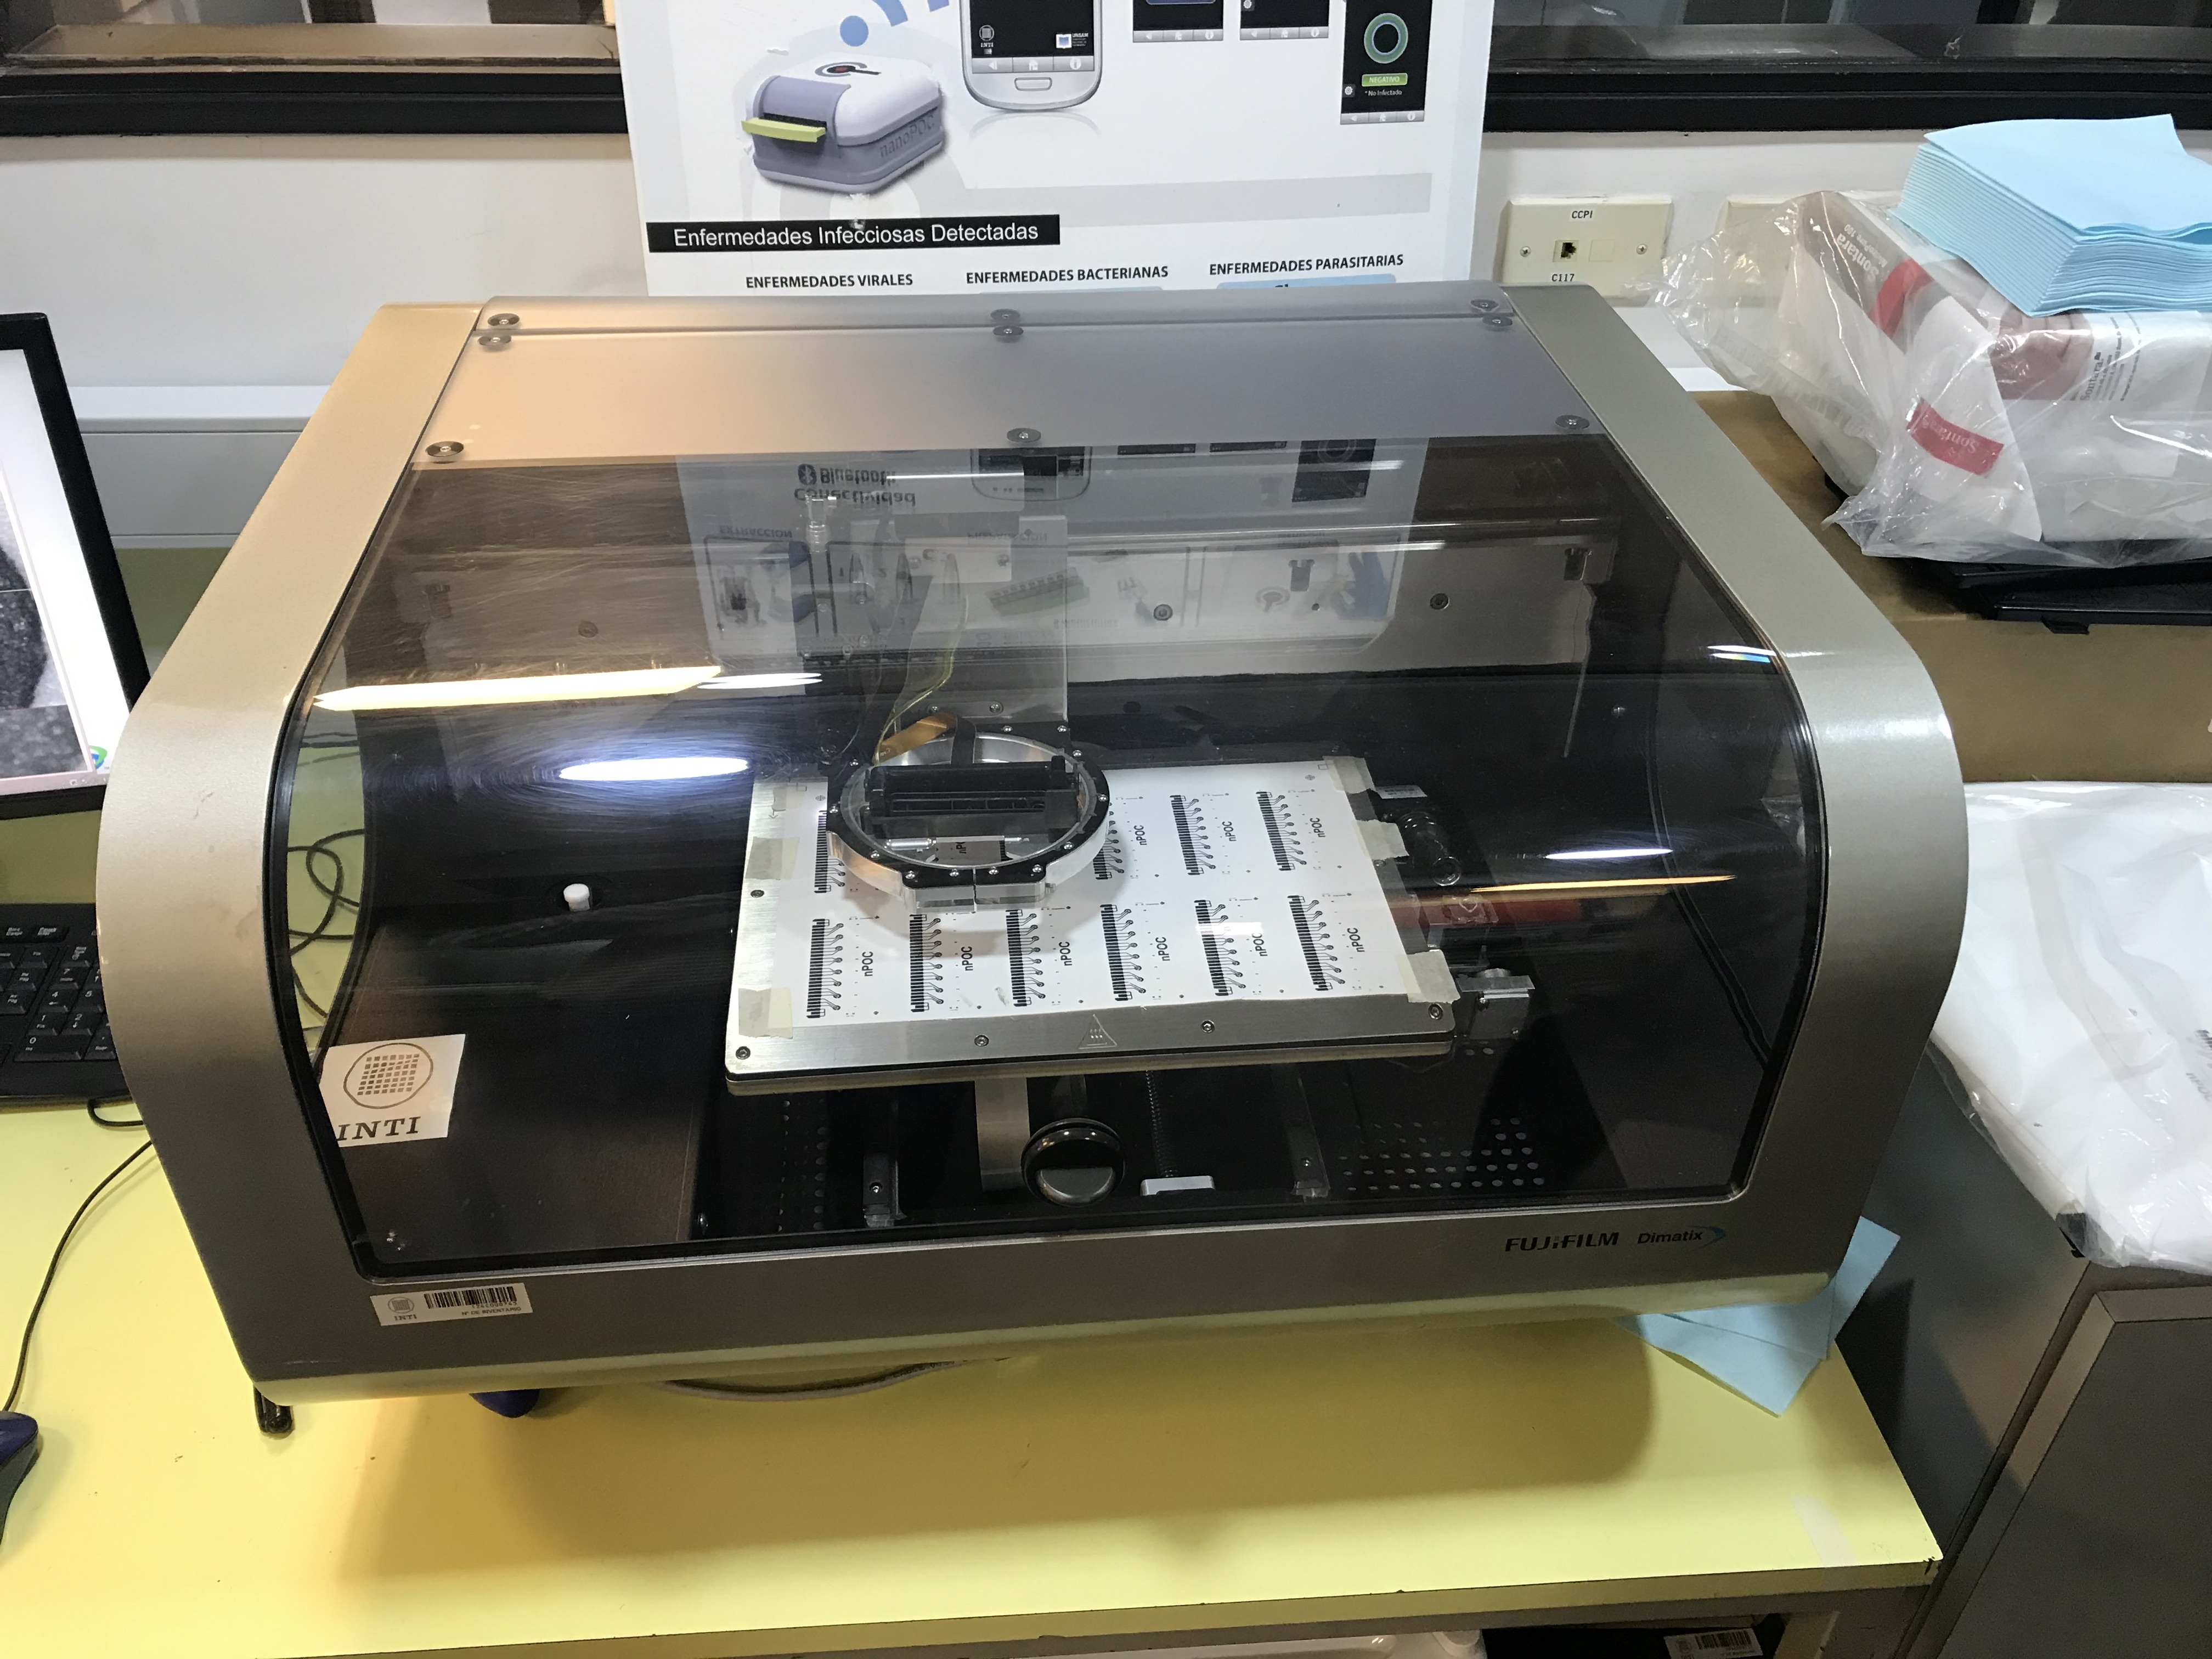
\includegraphics[width=0.5\textwidth]{Figures/Figura_Impresora_DMP2850}
  \caption{Fujifilm Dimatix DMP-2850 printer.}
  \label{fig:Figura_Impresora_DMP2850}
\end{figure}

The print head carrying base has a system to vary the angle of the ink cartridge and thus modify the distance between drops of the different ejectors (Figure ~\ref{fig:Figura_Carriage_angulo}) and a fiducial camera, which allows viewing the substrate and printing in real time and making measurements through the Software included with the printer (Figure ~\ref{fig:Figura_Vista_Camara_Fiducial}). 

\begin{figure}[H]
  \centering
    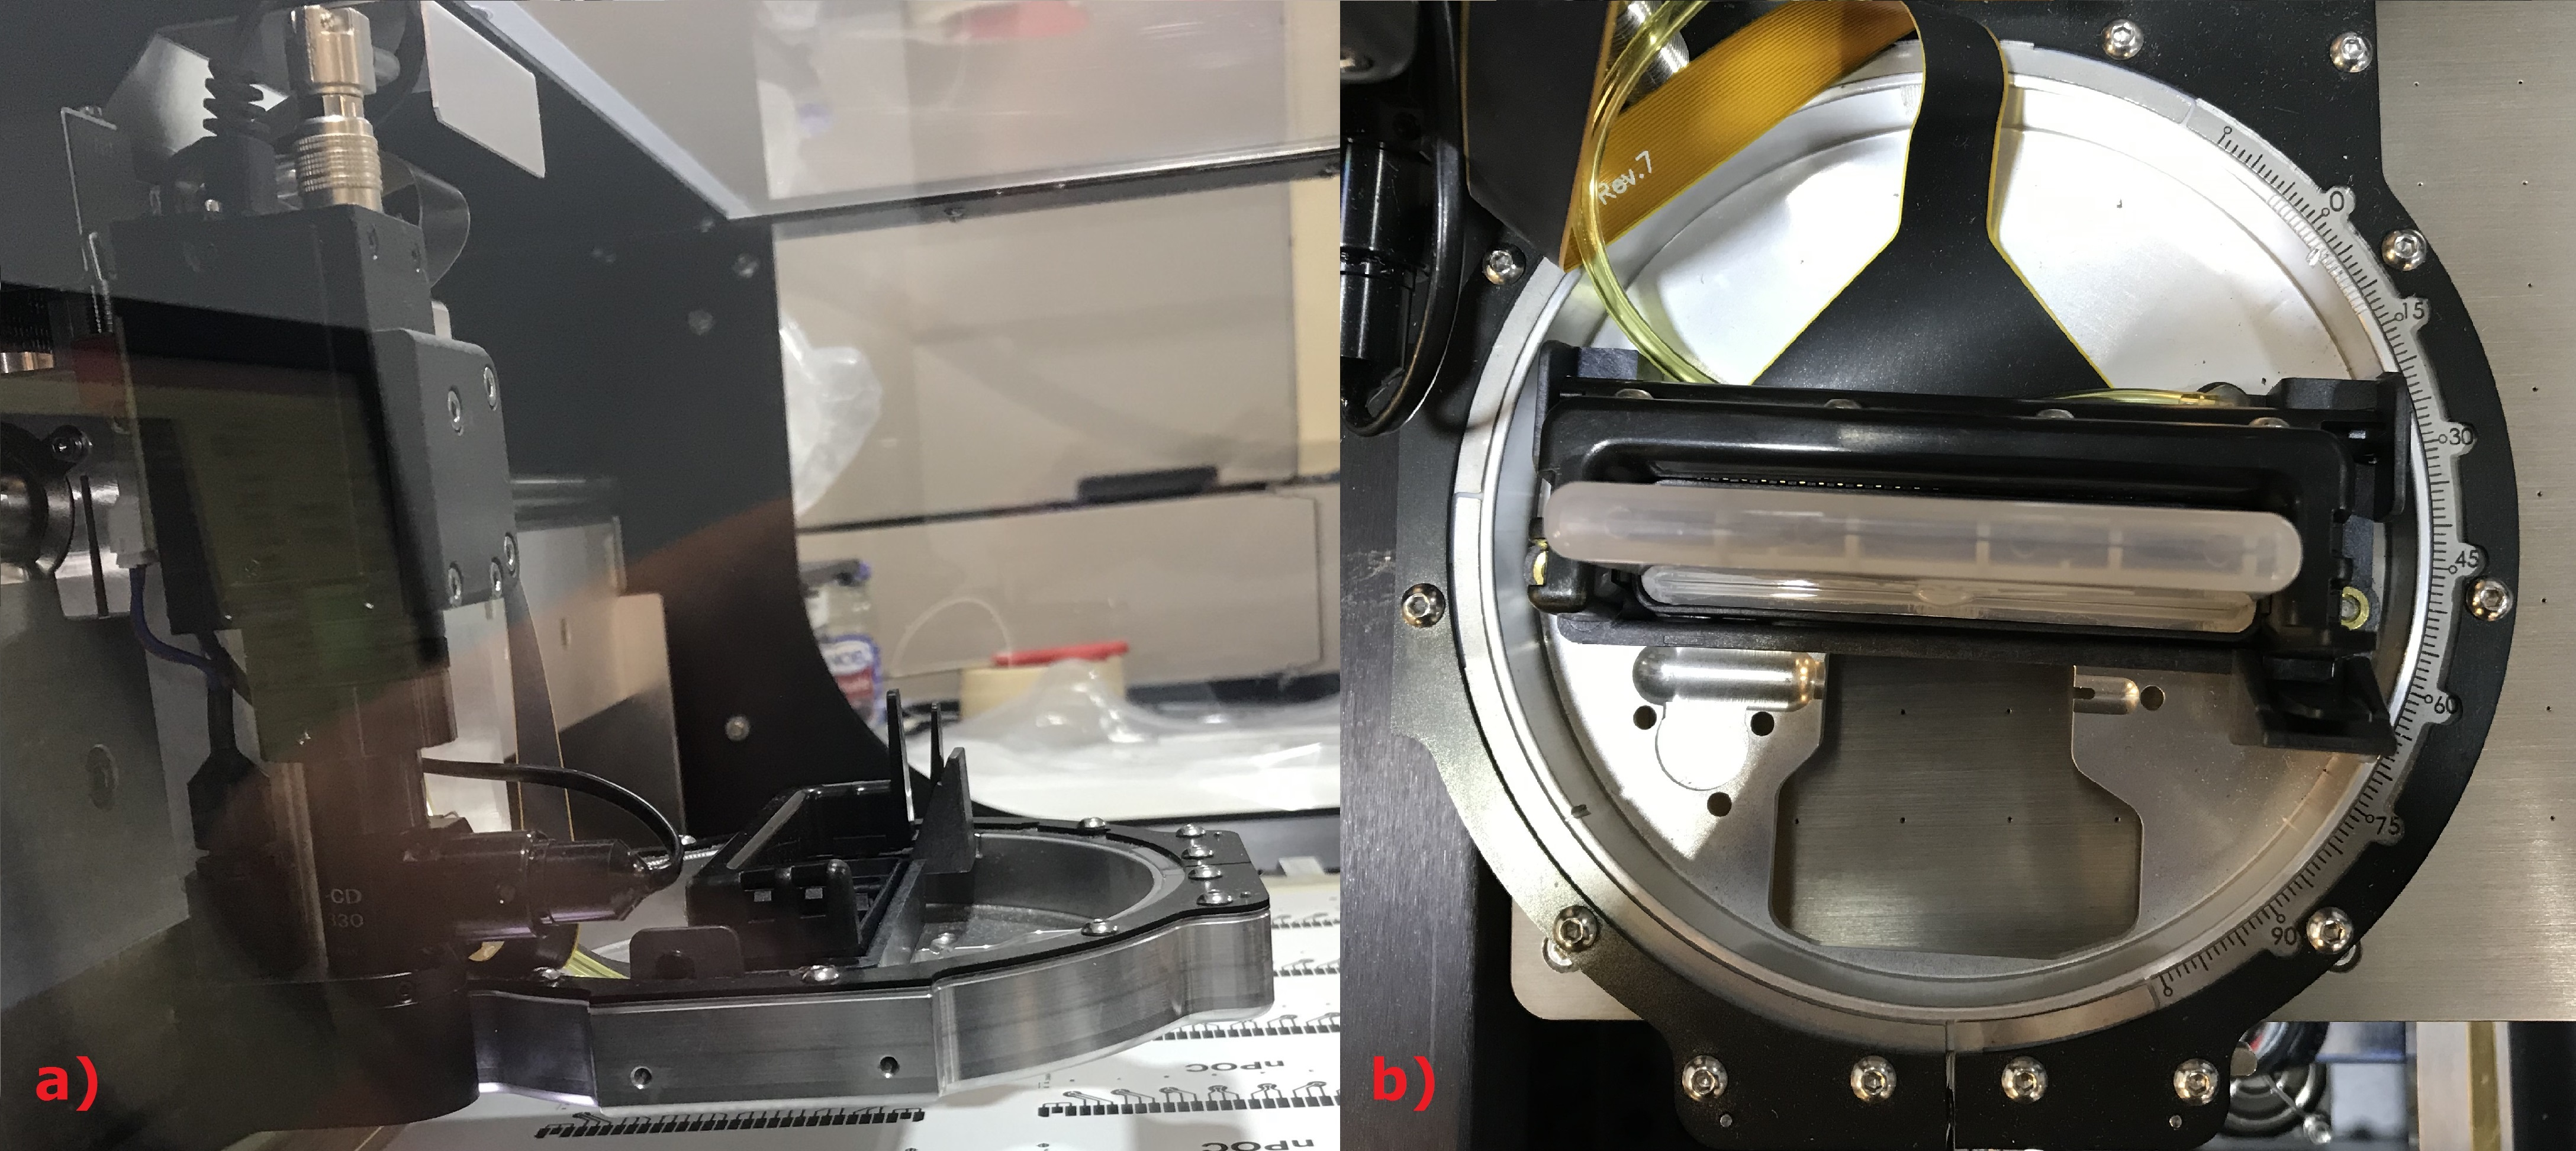
\includegraphics[width=0.8\textwidth]{Figures/Figura_Carriage_angulo}
  \caption{a) Print head carrying system b) System to modify the angle of the cartridge.}
  \label{fig:Figura_Carriage_angulo}
\end{figure}

\begin{figure}[H]
  \centering
    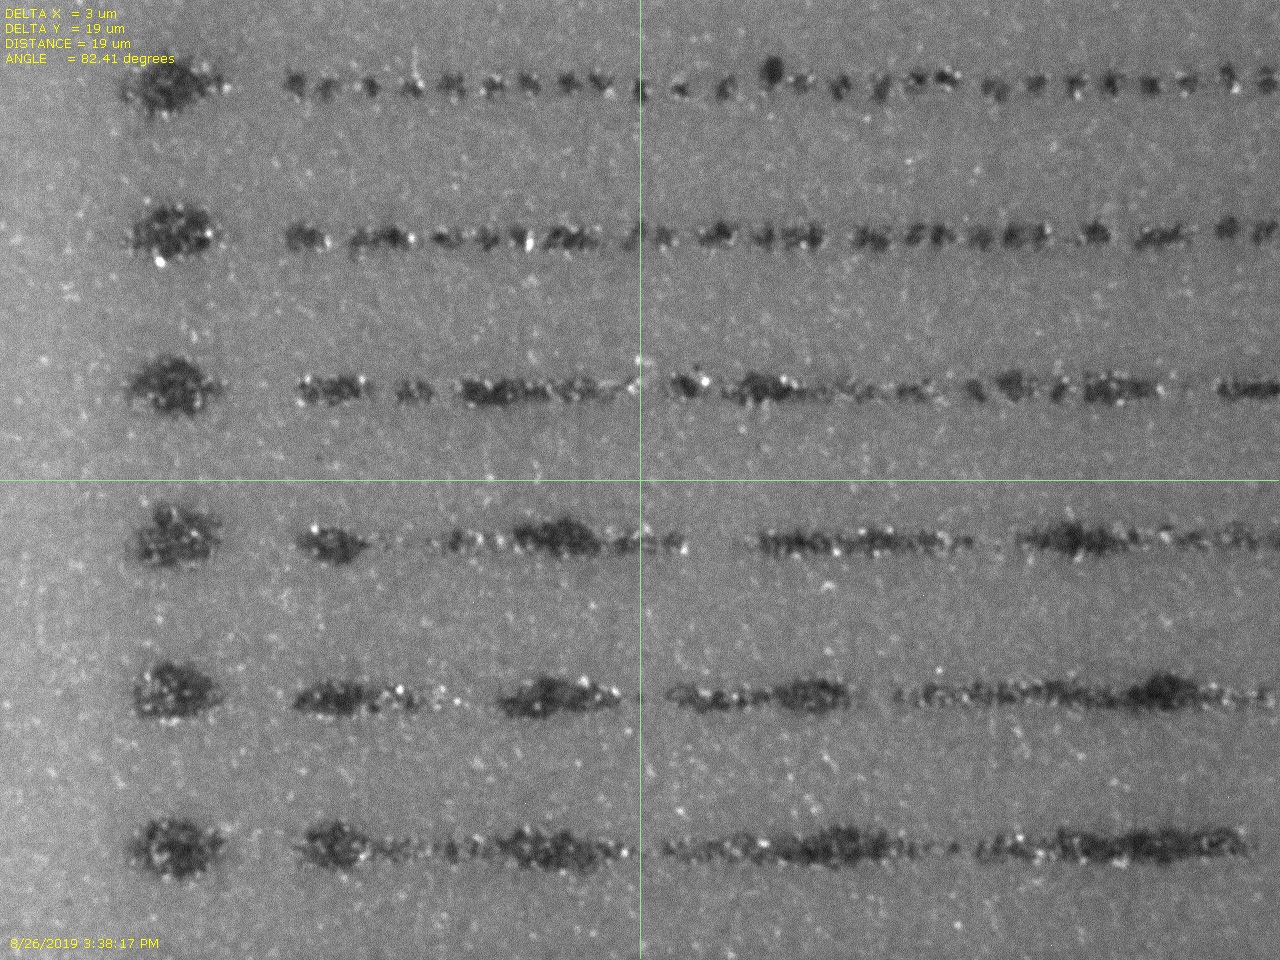
\includegraphics[width=0.5\textwidth]{Figures/Figura_Vista_Camara_Fiducial}
  \caption{Fiducial camera view from DMP Software.}
  \label{fig:Figura_Vista_Camara_Fiducial}
\end{figure}

To observe the status of the head, the ejection of the drops and to calibrate the printing system, the \textit{Drop Watcher} is used. This system consists of a camera oriented at 45º from the horizontal plane, with focus on the ejectors of the head (Figure ~\ref{fig:Figura_Drop_Watcher}). Using a strobe light, photographs or filming of the operation of each of the head holes can be taken (Figure ~\ref{fig:Figura_Drop_Watcher}).

\begin{figure}[H]
  \centering
    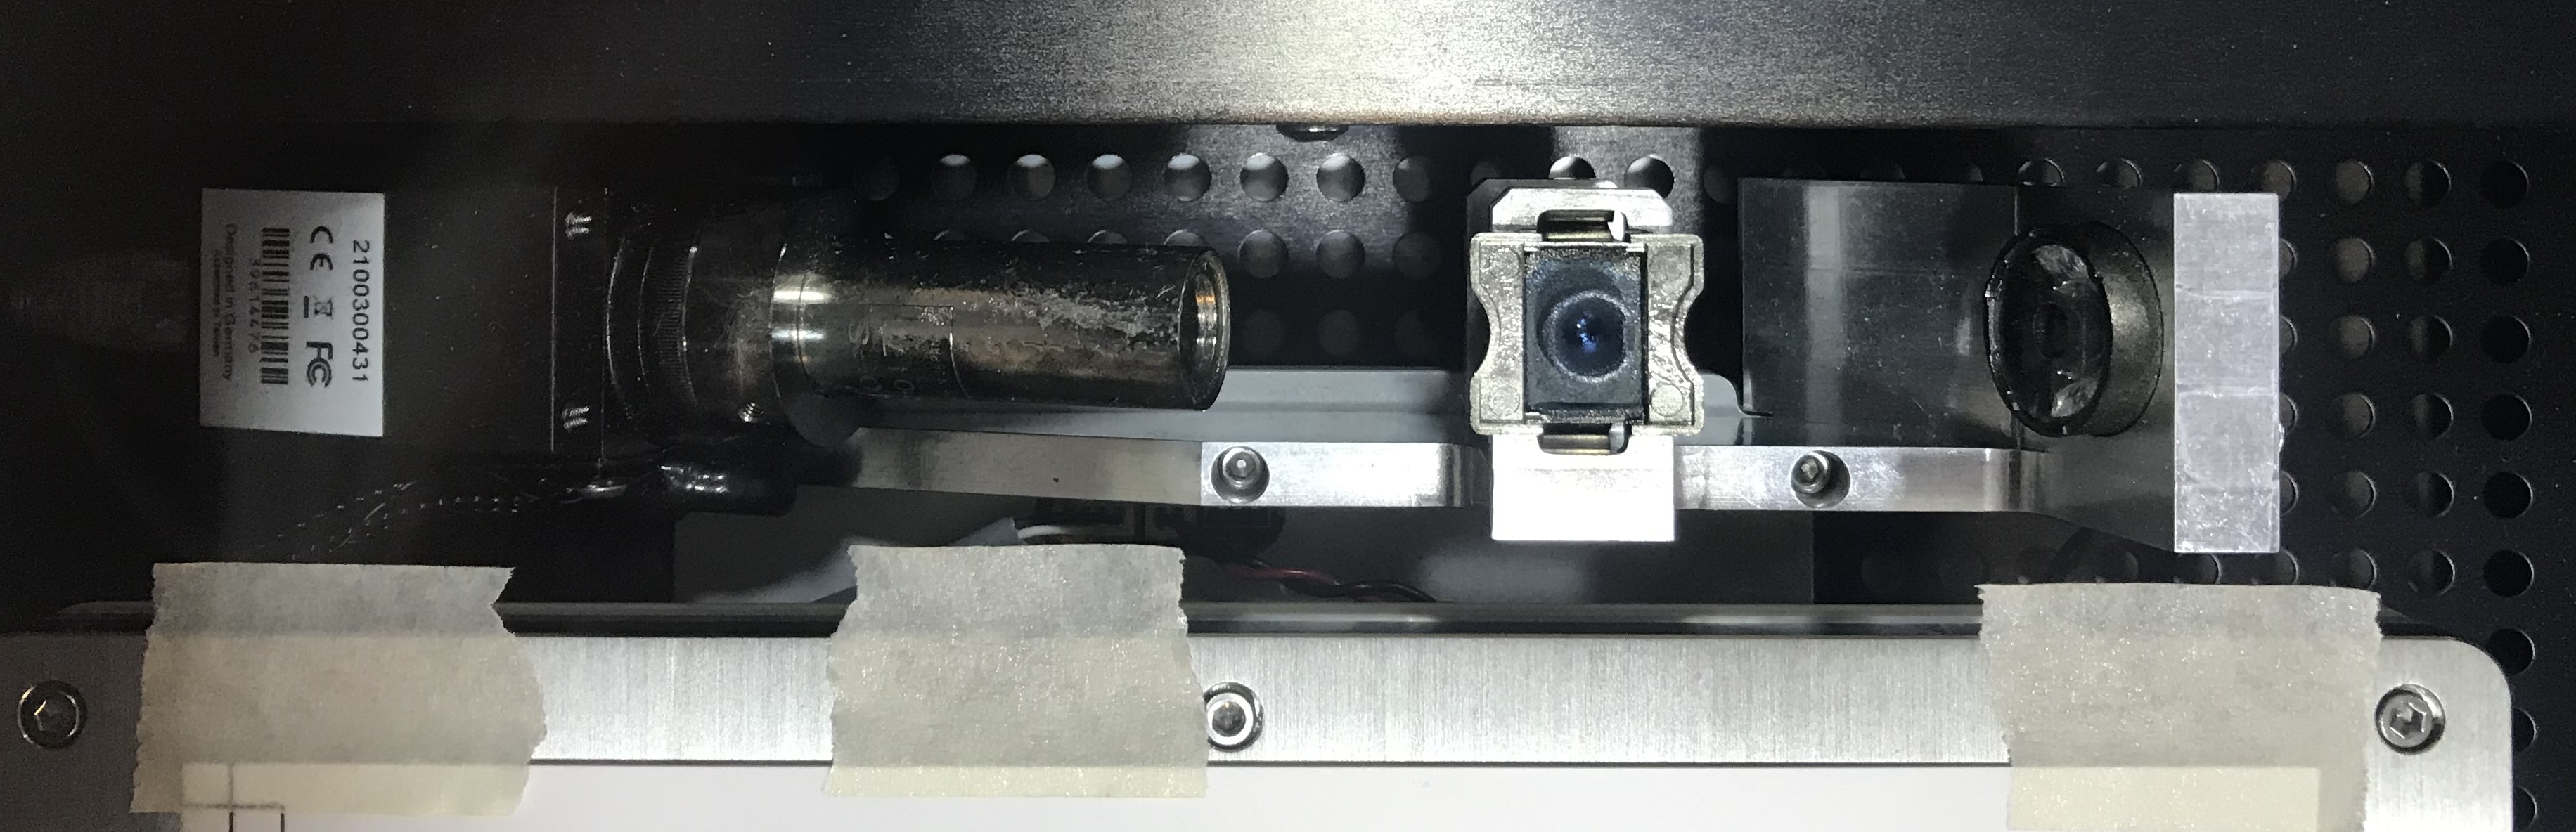
\includegraphics[width=0.5\textwidth]{Figures/Figura_Camara_Drop_Watcher}
  \caption{\textit{Drop Watcher} camera, light and reservoir system.}
  \label{fig:Figura_Camara_Drop_Watcher}
\end{figure}

\begin{figure}[H]
  \centering
    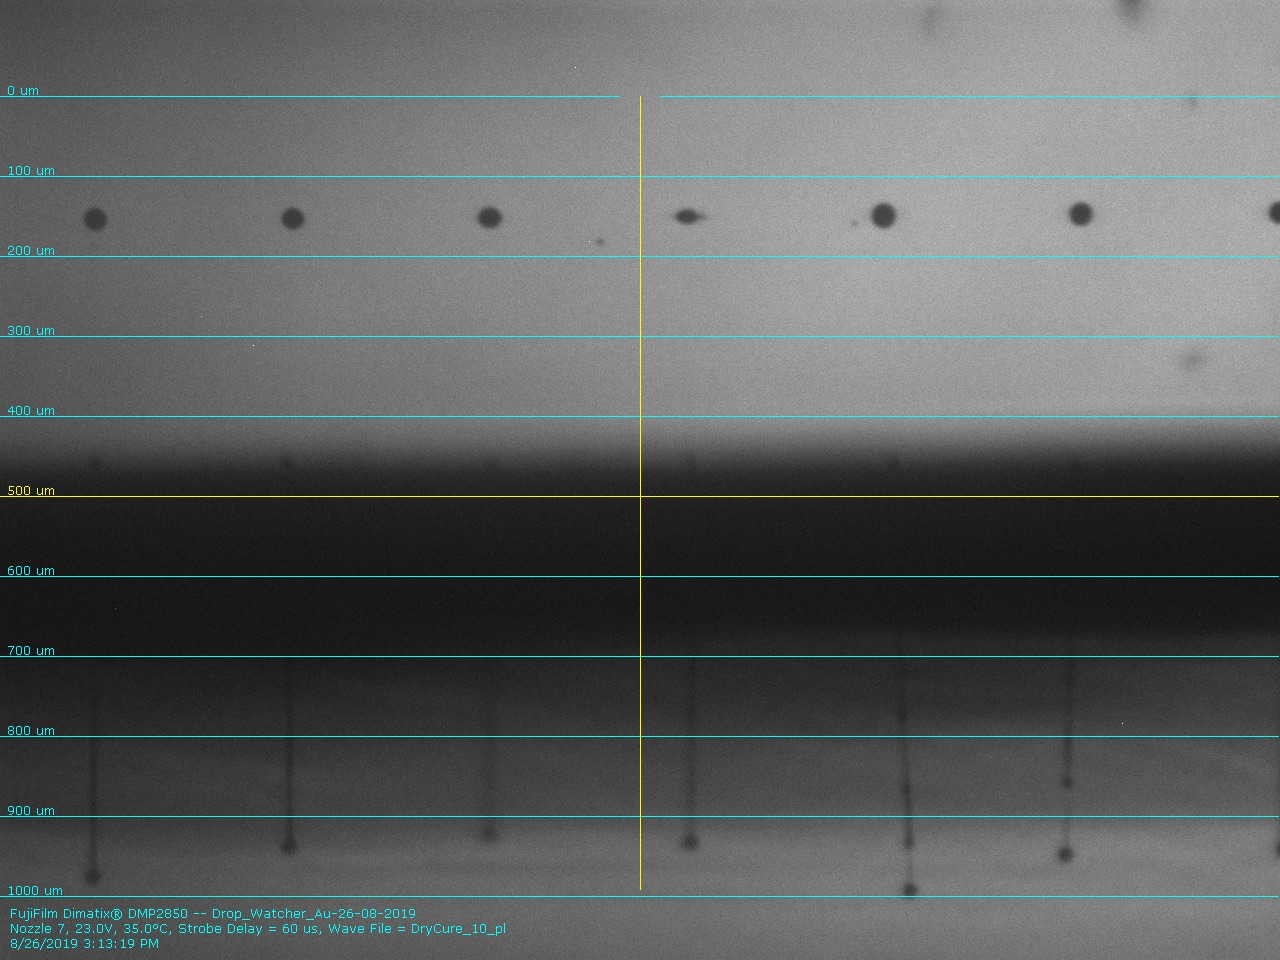
\includegraphics[width=0.5\textwidth]{Figures/Figura_Drop_Watcher}
  \caption{Image of drops being ejected using DMP Software.}
  \label{fig:Figura_Drop_Watcher}
\end{figure}

\section{Ink cartridge preparation}
Since the reservoirs and heads can only be used with one type of ink, Fujifilm offers them in the form of Printing Kits (Figure ~\ref{fig:Figura_kit_impresion}). Each Kit consists of a 3 ml reservoir, a head (depending on the model it can be 1 pl or 10 pl, referring to the volume of the drop ejected), a 3 ml syringe, a round tip needle and a $``$\textit{cleaning pad}$"$ Figure ~\ref{fig:Figura_Cleaning_pad}). The size of the syringe does not allow a larger volume of ink to be deposited than that supported by the reservoir system. The length of the needle prevents breakage of the cartridge container.

\begin{figure}[H]
  \centering
    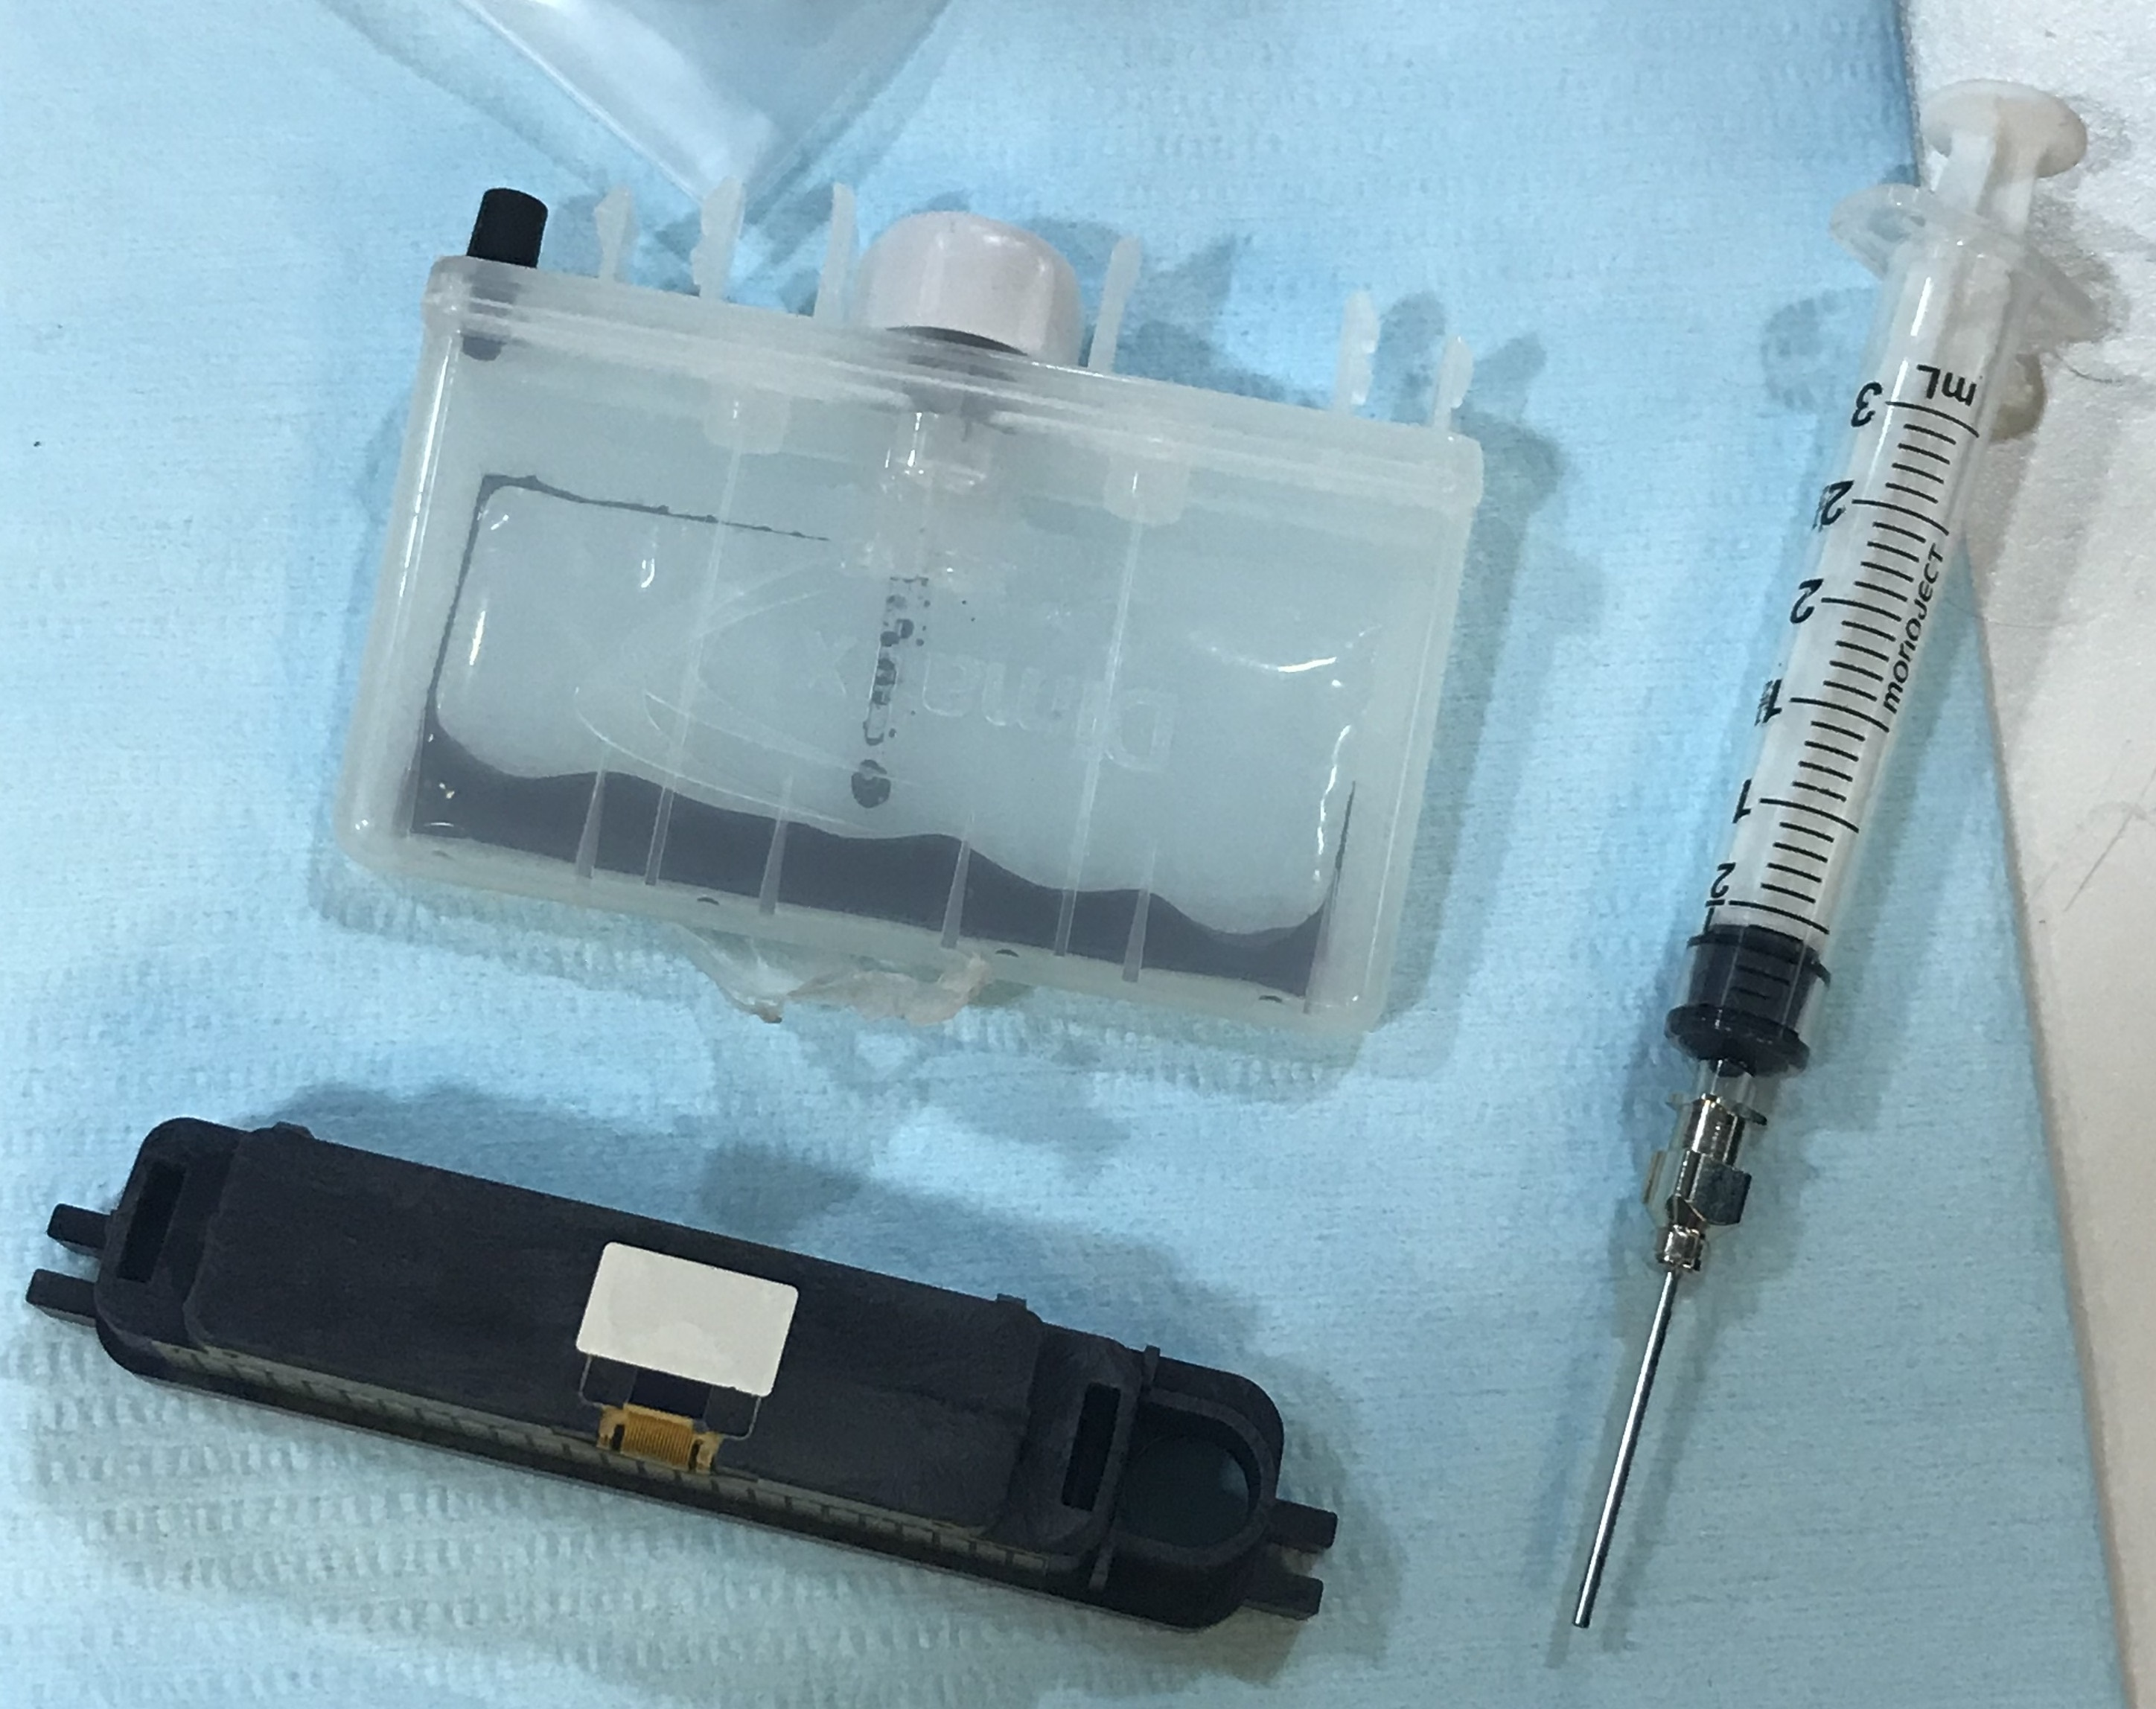
\includegraphics[width=0.5\textwidth]{Figures/Figura_kit_impresion}
  \caption{Print kit for Fujifilm Dimatix DMP2850 with 10 pl printhead filled with gold nanoparticles ink.}
  \label{fig:Figura_kit_impresion}
\end{figure}

\begin{figure}[H]
  \centering
    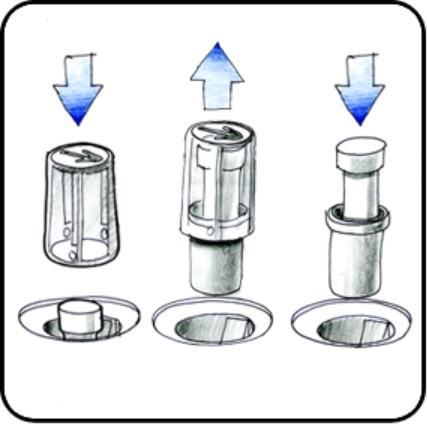
\includegraphics[width=0.5\textwidth]{Figures/Figura_Cleaning_pad}
  \caption{Usage of \textit{Cleaning Pad}.}
  \label{fig:Figura_Cleaning_pad}
\end{figure}

The \textit{Cleaning Pad} should be replaced once it is saturated with ink. This will be noticed by an excess of material on the substrate, the clogging of the ejectors or irregularities in the printing, such as misalignment of the drops on the substrate. To check if it is ink deposited on the head, the \textit{Drop Watcher} is used, where you can easily see the state of the ejectors and the flight of the drops (Figure ~\ref{fig:Figura_suciedad_cabezal}).

\begin{figure}[H]
  \centering
    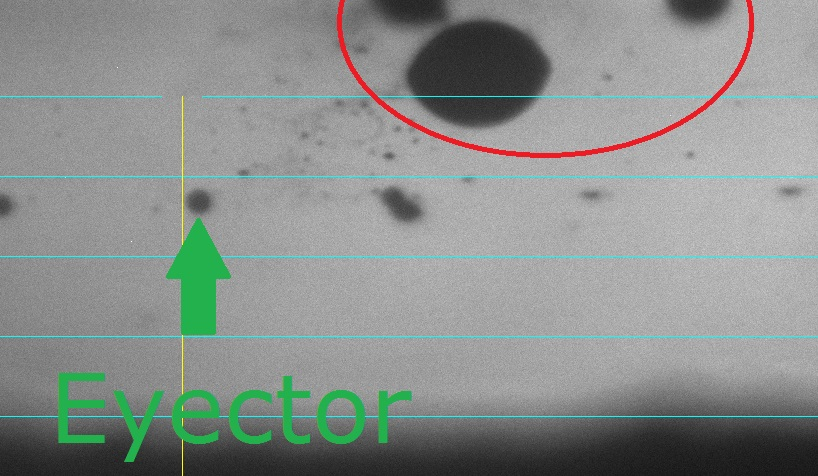
\includegraphics[width=0.5\textwidth]{Figures/Figura_suciedad_cabezal}
  \caption{Ink deposited on the head due to the saturated \textit{Cleaning Pad}.}
  \label{fig:Figura_suciedad_cabezal}
\end{figure}

In the first instance, the quantity of ink to be used with the syringe is taken and deposited inside the reservoir. The length of the needle does not allow reaching the end of the reservoir, preventing perforation (Figure ~\ref{fig:Figura_carga_tinta}).

\begin{figure}[H]
  \centering
    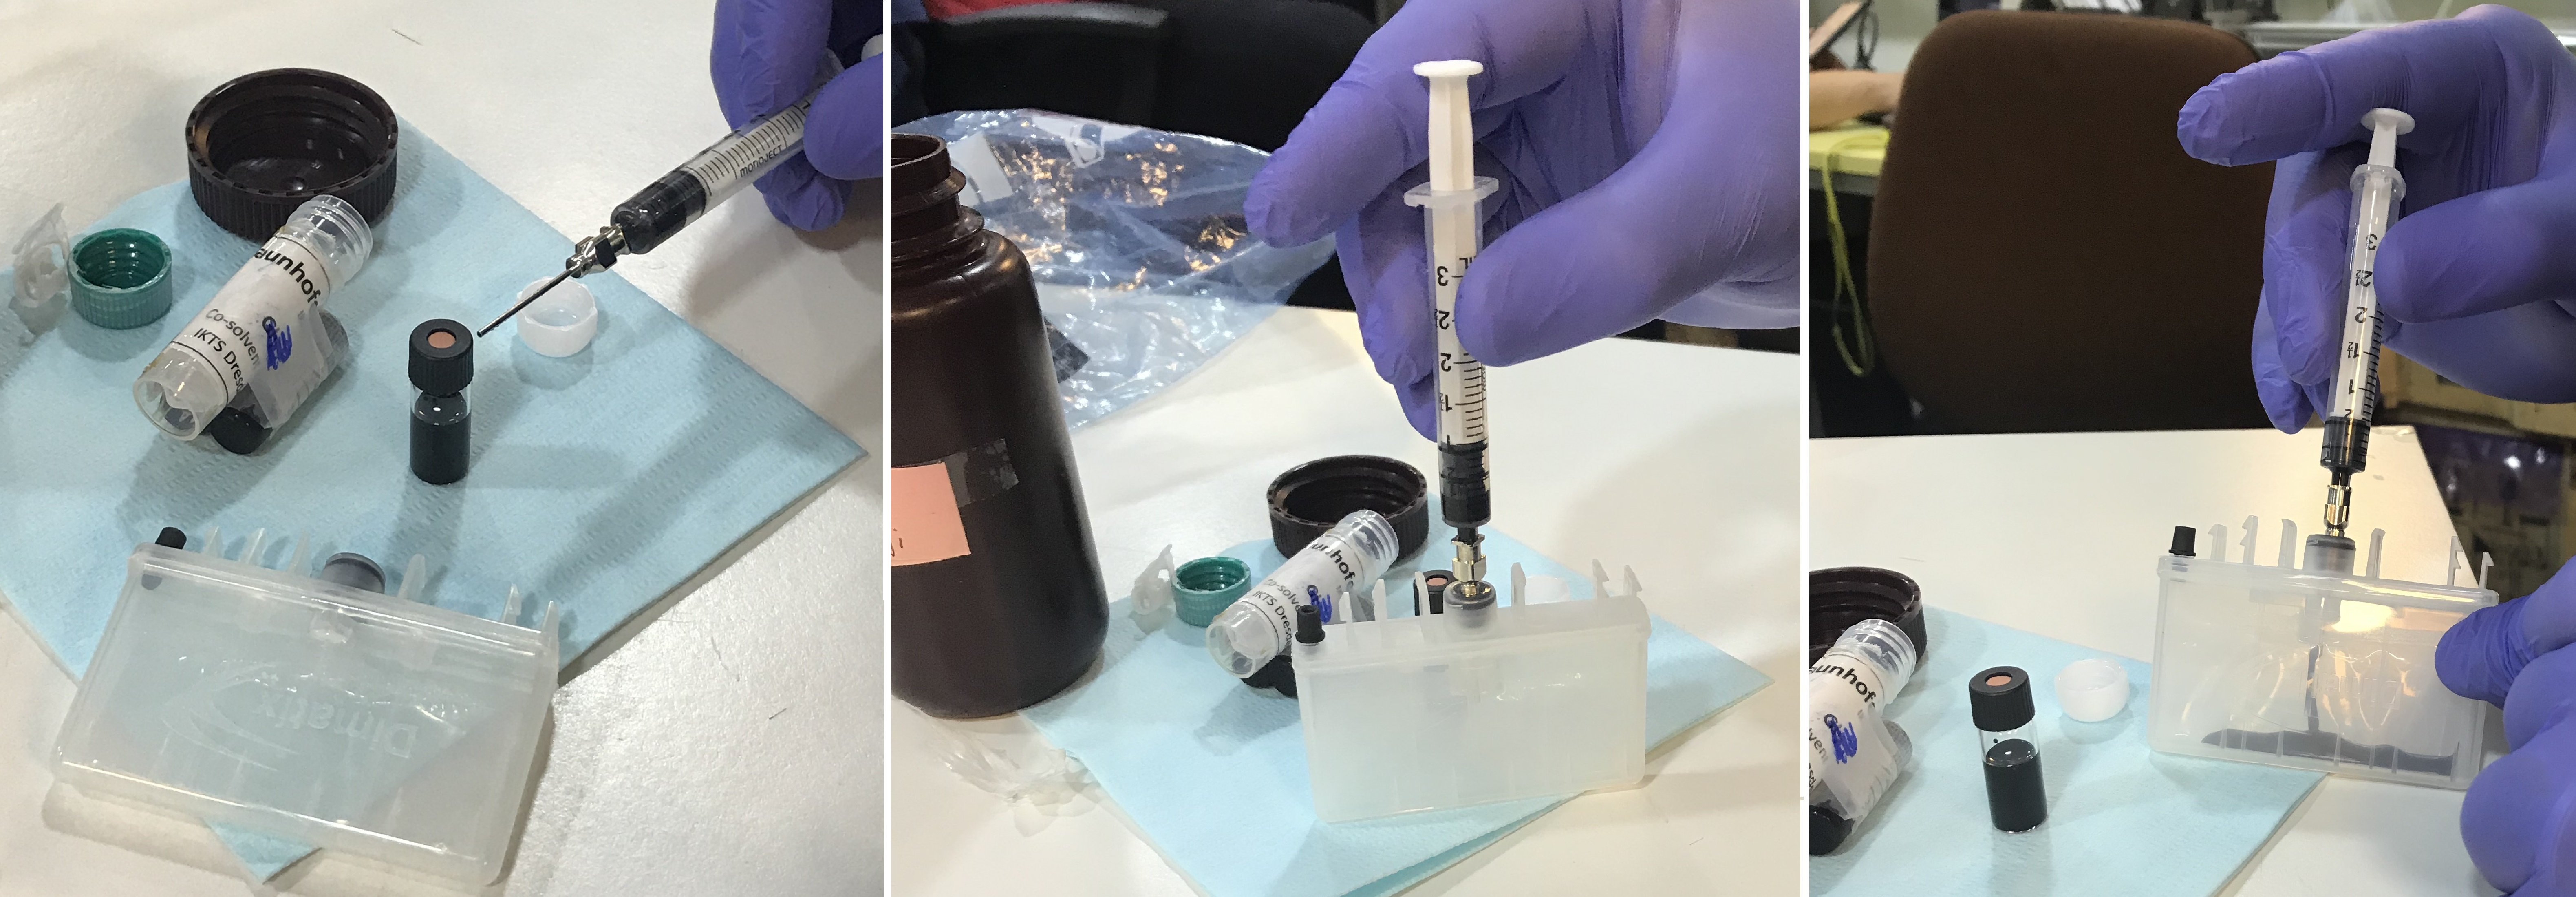
\includegraphics[width=1\textwidth]{Figures/Figura_carga_tinta}
  \caption{Reservoir filling procedure.}
  \label{fig:Figura_carga_tinta}
\end{figure}

Once the reservoir is filled with the desired ink, the reservoir is installed over the head. Since it has a connection to a pressure line to generate a vacuum inside by helping the ink movement, the cartridge can only be assembled in one direction. According to Fujifilm's recommendations, it should be adjusted first on the side of the vacuum connector, pressing until you hear a $``$\textit{click}$"$, then check that the ink tank is aligned with the head and force it again until you hear a second $``$\textit{click}$"$. In this way, the ink tank is anchored to the head.

The cartridge must be inserted into the reel (Figure ~\ref{fig:Figura_Carrete1}) keeping in mind that the correct orientation is that which allows the head contacts to be aligned with those of the reel. For this the printer must be turned on and the \textit{Dimatix Drop Manager} Software running with its complete initial checkup procedure.

\begin{figure}[H]
  \centering
    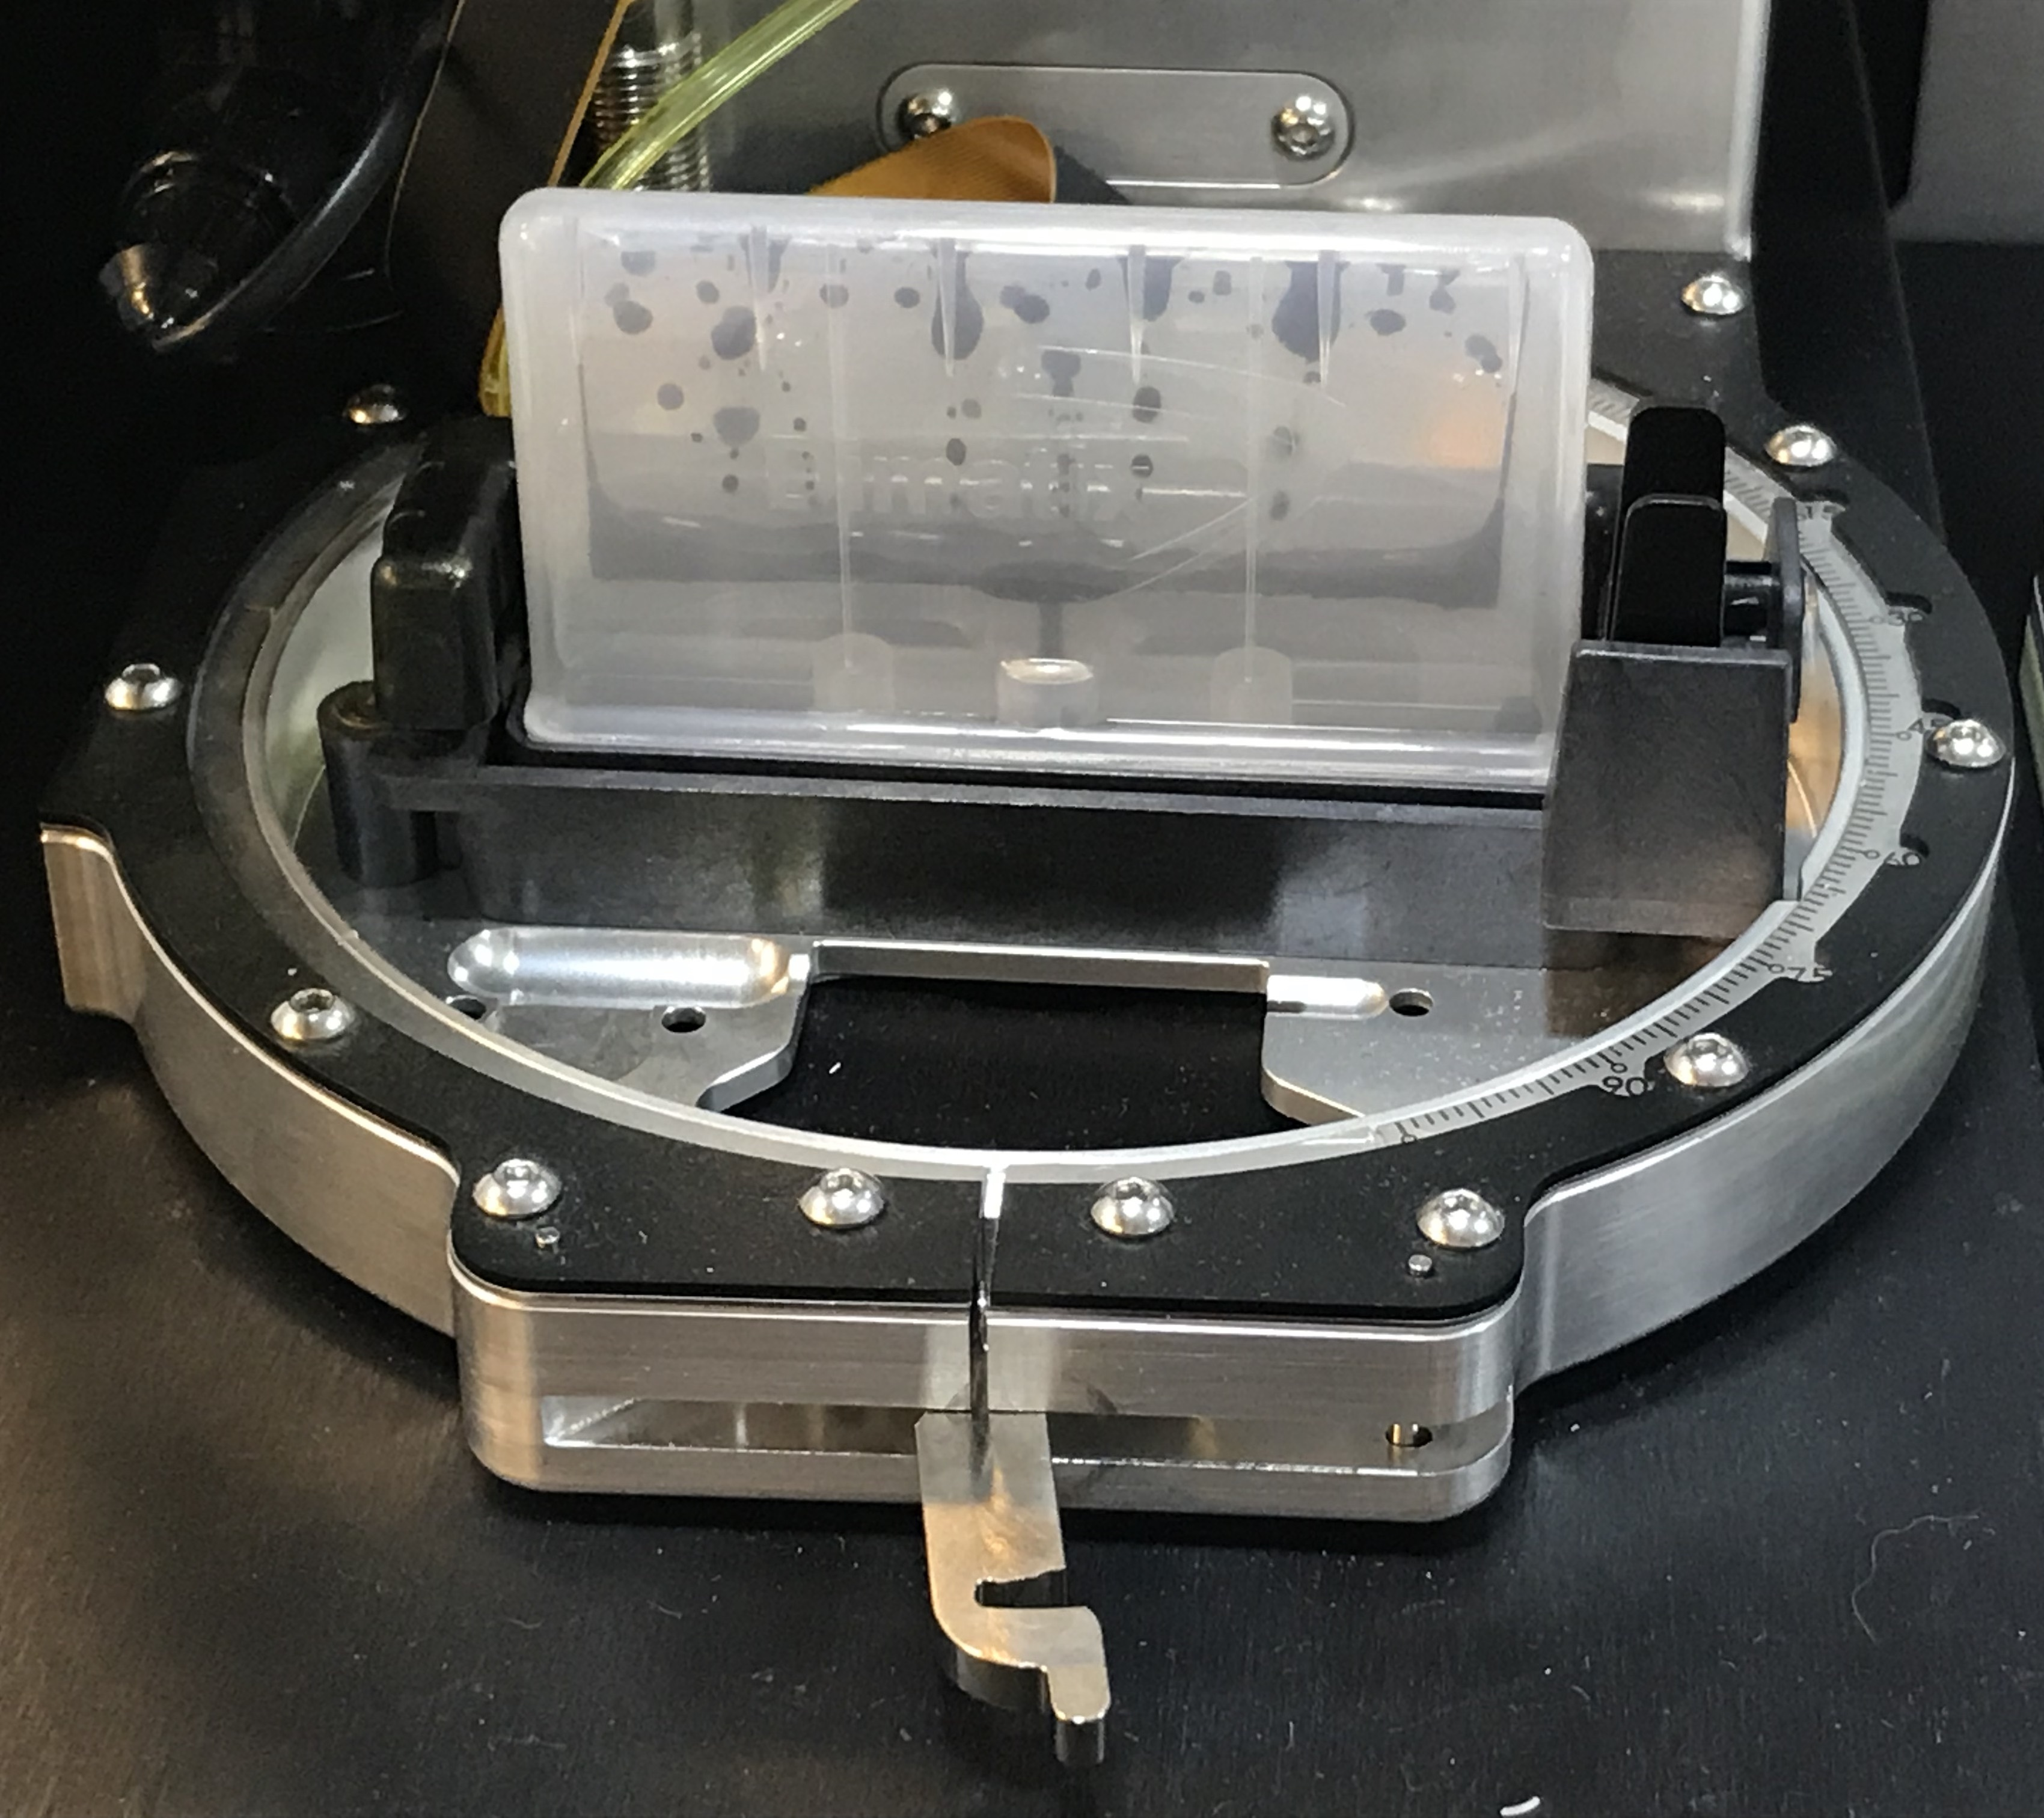
\includegraphics[width=0.5\textwidth]{Figures/Figura_Carrete1}
  \caption{Reel with the cartridge is installed.}
  \label{fig:Figura_Carrete1}
\end{figure}

Once the cartridge is installed, the \textit{Cleaning Pad} is placed in the dedicated hole for this object (Figure ~\ref{fig:Figura_Orificio_Cleaning_Pad}). This should be done before closing the cartridge installation procedure to avoid spilling ink on the reel rest base.

\begin{figure}[H]
  \centering
    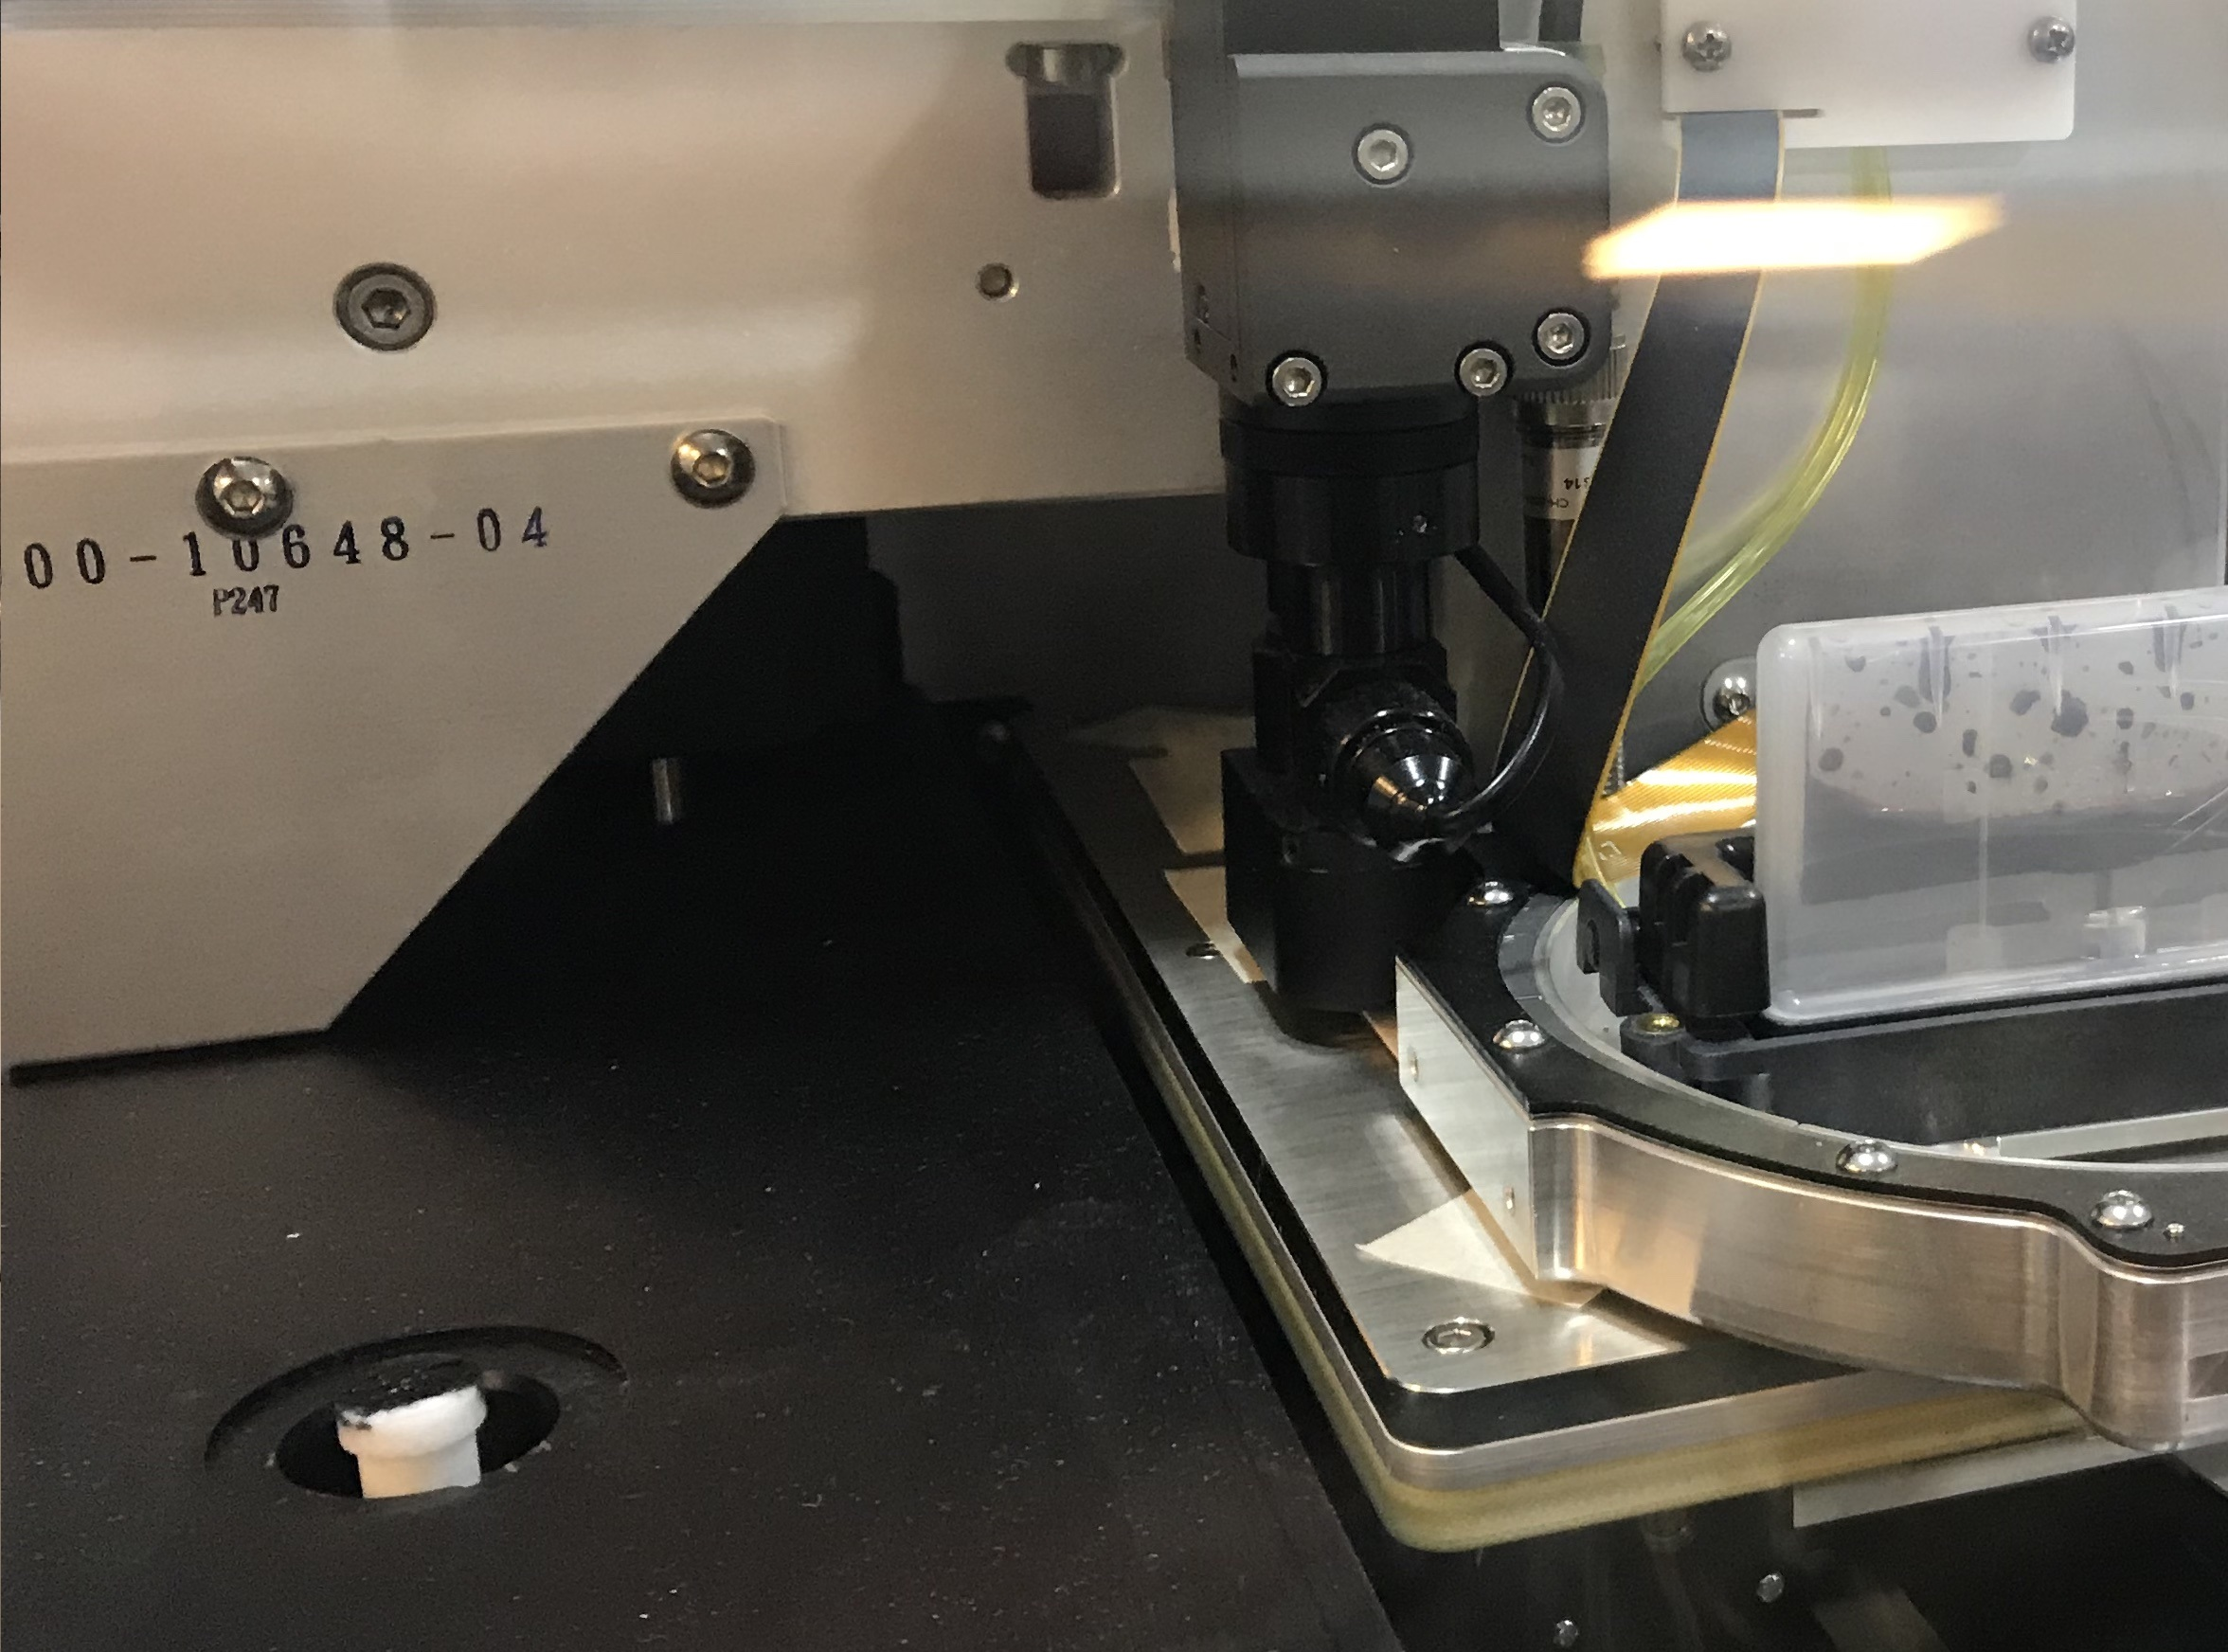
\includegraphics[width=0.5\textwidth]{Figures/Figura_Orificio_Cleaning_Pad}
  \caption{\textit{Cleaning Pad} location.}
  \label{fig:Figura_Orificio_Cleaning_Pad}
\end{figure}

By closing the printer cover, the cartridge installation procedure is completed and the software asks to load the configuration file, which is unique for each ink. Within this file is the waveform that handles the ejectors (Figure ~\ref{fig:Figura_Pantalla_Waveform}) and the parameters adjusted so that the formation and deposition of the drops of the material is possible. Within these parameters are the upper limit of voltage for each ejector, the temperature of the head, the vacuum pressure to generate the ink meniscus, the height at which the cartridge will move with respect to the substrate and the cleaning cycles before, during and after printing (Figure ~\ref{fig:Figura_Configuraciones_cartucho}).

\begin{figure}[H]
  \centering
    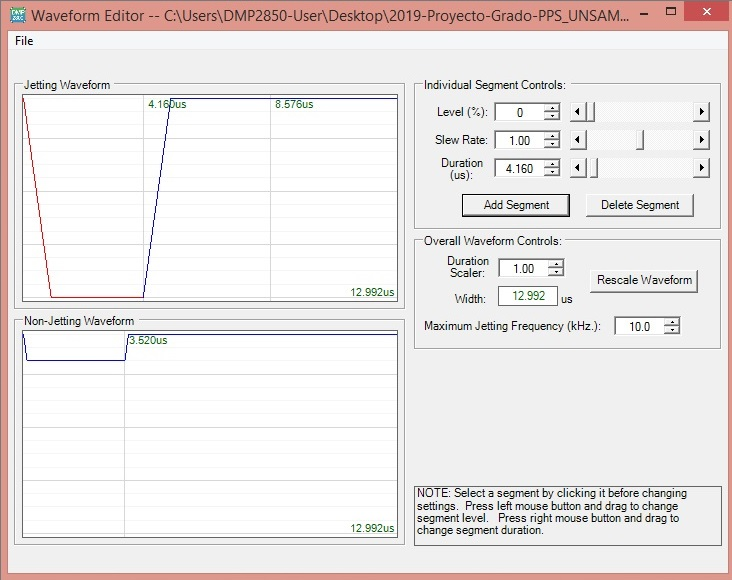
\includegraphics[width=0.5\textwidth]{Figures/Figura_Pantalla_Waveform}
  \caption{Setup screen with Waveform.}
  \label{fig:Figura_Pantalla_Waveform}
\end{figure}

\begin{figure}[H]
  \centering
    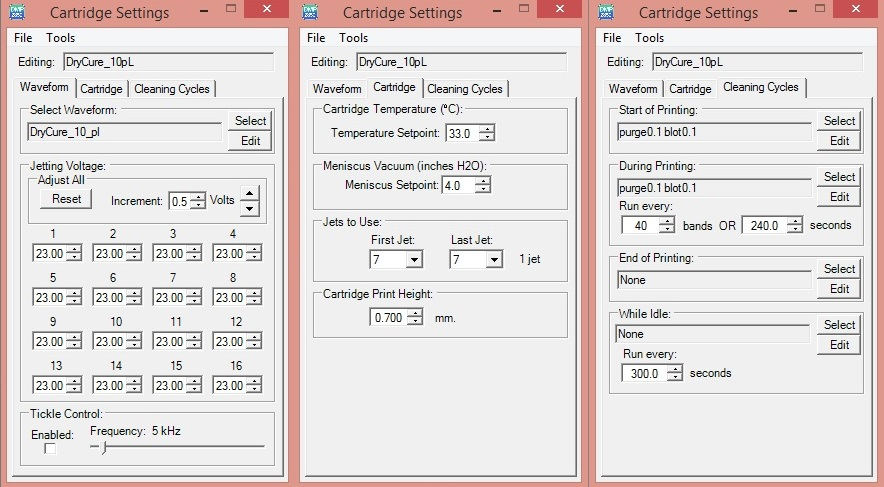
\includegraphics[width=0.8\textwidth]{Figures/Figura_Configuraciones_cartucho}
  \caption{Screens for setting of the printing parameters.}
  \label{fig:Figura_Configuraciones_cartucho}
\end{figure}

To check the correct operation of the system, the \textit{Drop Watcher} is used where the ejection of the drops from the configured \textit{nozzles} can be seen in real time and, at the same time, the voltage adjustment can be made to match the flight time of the different ejectors (Figure ~\ref{fig:Figura_drop_watcher1}).

\begin{figure}[H]
  \centering
    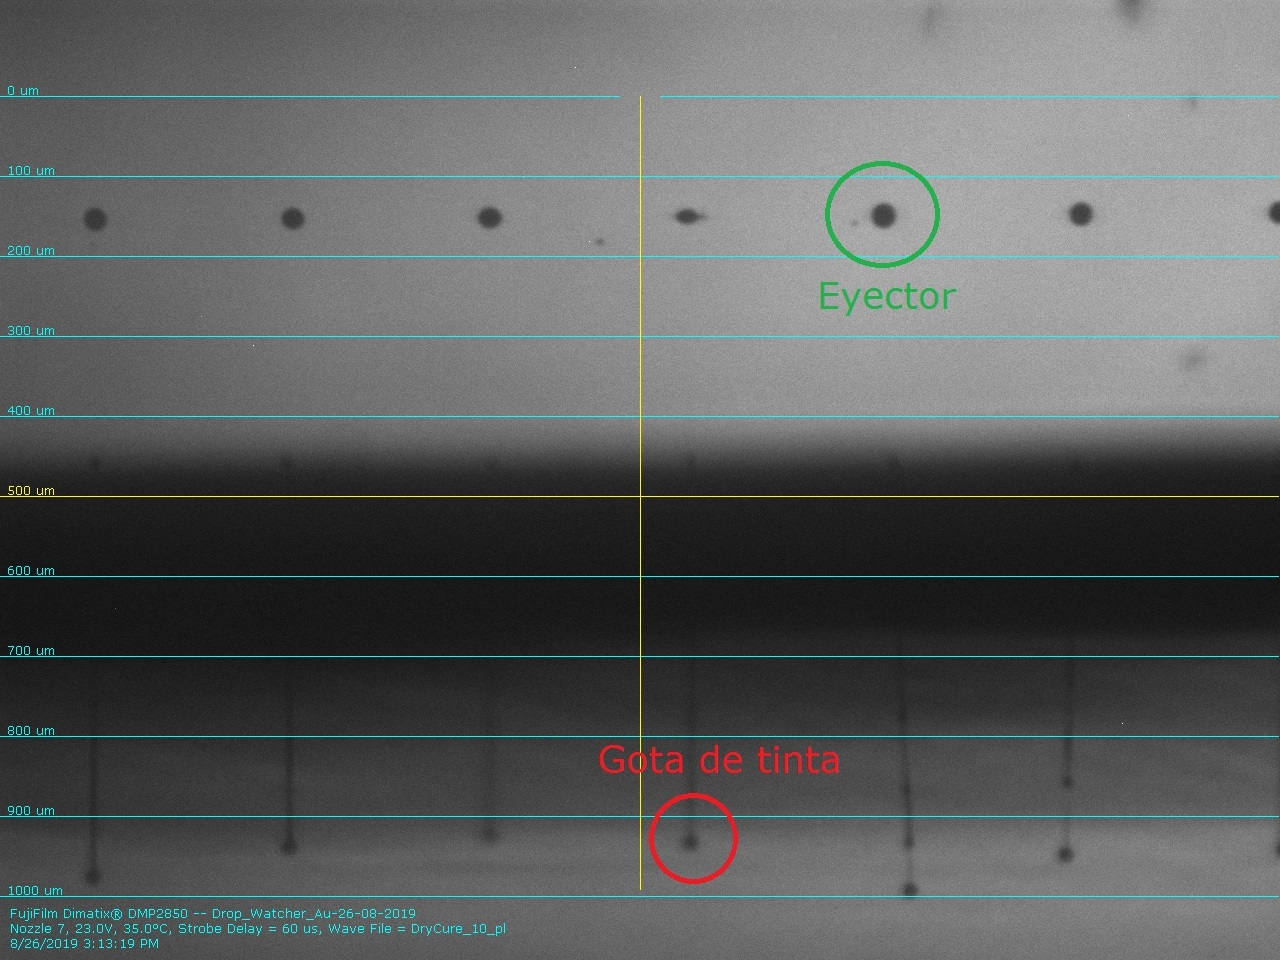
\includegraphics[width=0.5\textwidth]{Figures/Figura_drop_watcher1}
  \caption{Drop Watcher screen.}
  \label{fig:Figura_drop_watcher1}
\end{figure}

Once the use of the cartridge is finished, it must be placed vertically, otherwise the channel that feeds the head will empty of ink (Figure ~\ref{fig:Figura_canal_cartucho_vacio}). If this happens, several purge cycles must be carried out or fill with more ink, but there is no guarantee that the cartridge will work properly again.

\begin{figure}[H]
  \centering
    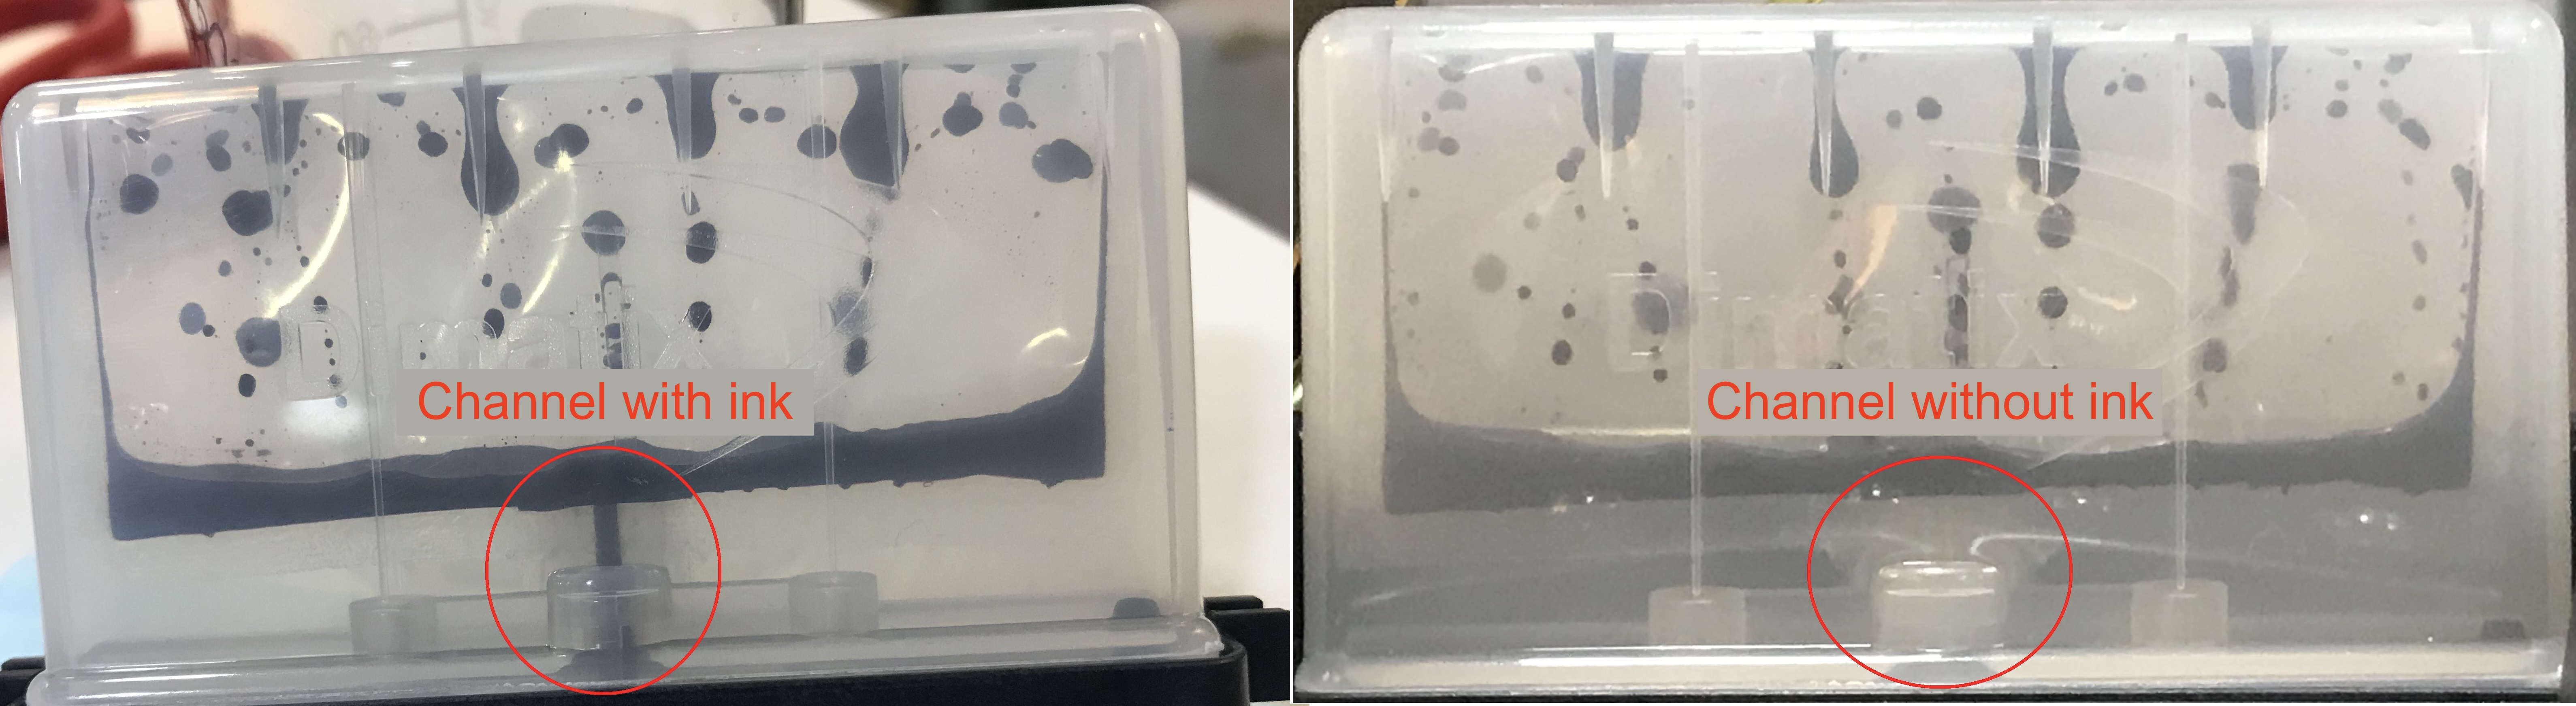
\includegraphics[width=1\textwidth]{Figures/Figura_canal_cartucho_vacio}
  \caption{Cartridge channel without ink.}
  \label{fig:Figura_canal_cartucho_vacio}
\end{figure}

\section{Substrate clamping and platen configuration}
The printer platen is a metal surface with an arrangement of holes where a vacuum is generated to suck the substrate on which is wanted to print (Figure ~\ref{fig:Figura_platina}). Although the vacuum generated in the holes is considerable, special attention must be paid to ensure that the entire surface is in contact, otherwise the clamping will not be sufficient to keep the substrate fixed at the time of printing. If all the holes are not obstructed by the substrate, the system will not generate the negative pressure stipulated by the manufacturer and the fixing will not be assured.

\begin{figure}[H]
  \centering
    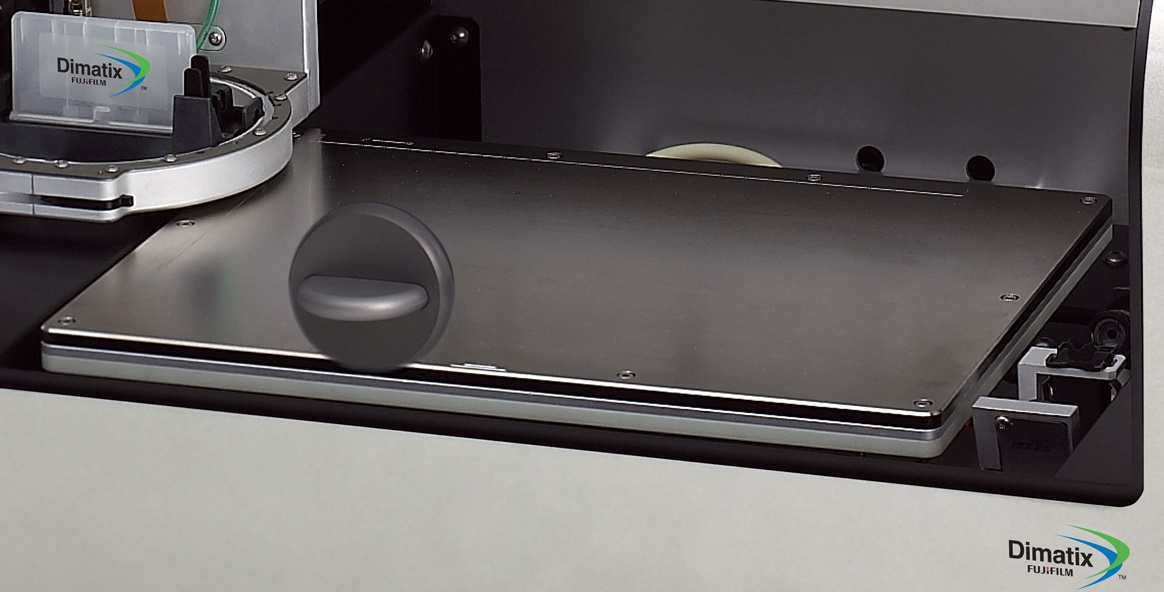
\includegraphics[width=0.5\textwidth]{Figures/Figura_platina}
  \caption{Fujifilm Dimatix DMP-2850 Printer platen.}
  \label{fig:Figura_platina}
\end{figure}

To prevent these problems and ensure the correct anchorage of the surface to be printed, adhesive paper tape is used.

It is important that the base to be printed does not move during the entire printing process, paying the greatest attention after performing the \textit{Theta} calibration, explained in the section on Commissioning and calibration of the printer, since it compensates the angular \textit{offset} that can be generated between the substrate once fixed and the platen.

Once the substrate has been positioned and anchored, the thickness of the substrate and the temperature of the platen must be configured using the printer software. If adhesive tape was used to place the sample, it is advisable to add a greater thickness to avoid spool rubbing, ink loss, or head breakage.